\documentclass[10pt, a4paper]{article}

\usepackage{mathtext}
\usepackage[T1,T2A]{fontenc}
\DeclareSymbolFont{T2Aletters}{T2A}{cmr}{m}{it} 
\usepackage[utf8]{inputenc}
\usepackage[english,russian]{babel}
\usepackage{graphicx,amsmath,color,listings}
\usepackage[margin=1in]{geometry}

\title{Курсовая работа по предмету "Базы данных"}
\author{Андрей Козлов, гр. 4538}
\date{25 января 2013г.}

\begin{document}
\maketitle

\section{Постановка задачи}

Некоторая компания предоставляет своим сотрудникам возможность бесплатно общаться по мобильному телефону. Для этого был заключен контракт с оператором мобильной связи на следующих условиях:
\begin{itemize}
	\item компании выдается набор корпоративных номеров, общение между которыми не тарифицируется;
	\item цены на все остальные услуги устанавливаются в соответствии с действующими тарифами оператора.
\end{itemize}

Сотрудник компании может заключить договор на использование корпоративного номера. В договоре указывается тариф оператора, по которому будут тарифицироваться услуги. Один сотрудник может иметь более одного номера в любой момент времени.

Чтобы контролировать расходы компании на мобильную связь, требуется реализовать биллинговую систему, умеющую выполнять следующие операции:
\begin{itemize}
	 \item добавить новый корпоративный номер;
	\item добавить нового сотрудника;
	\item заключить контракт с сотрудником на использование корпоративного номера с указанным тарифным планом;
	\item расторгнуть контракт с сотрудником на использование корпоративный номер;
	\item сменить тарифный план контракта;
	\item расчитать расходы сотрудника за заданный период;
	\item расчитать все расходы сотрудника;
	\item вычислить процент расходов на личные разговоры.
\end{itemize}

Данная курсовая работа представляет собой реализацию такой биллинговой системы.

\section{Модель}

Список сущностей:
\begin{itemize}
	\item сотрудник;
	\item номер корпоративного телефона;
	\item тарифный план оператора;
	\item услуга (звонок, sms/mms-сообщение, gprs-соединение и т.д.);
	\item единица тарификации услуги (секунды, штуки, кБ и т.д.);
	\item мобильная операция.
\end{itemize}

\begin{figure}[H]
	\centering
	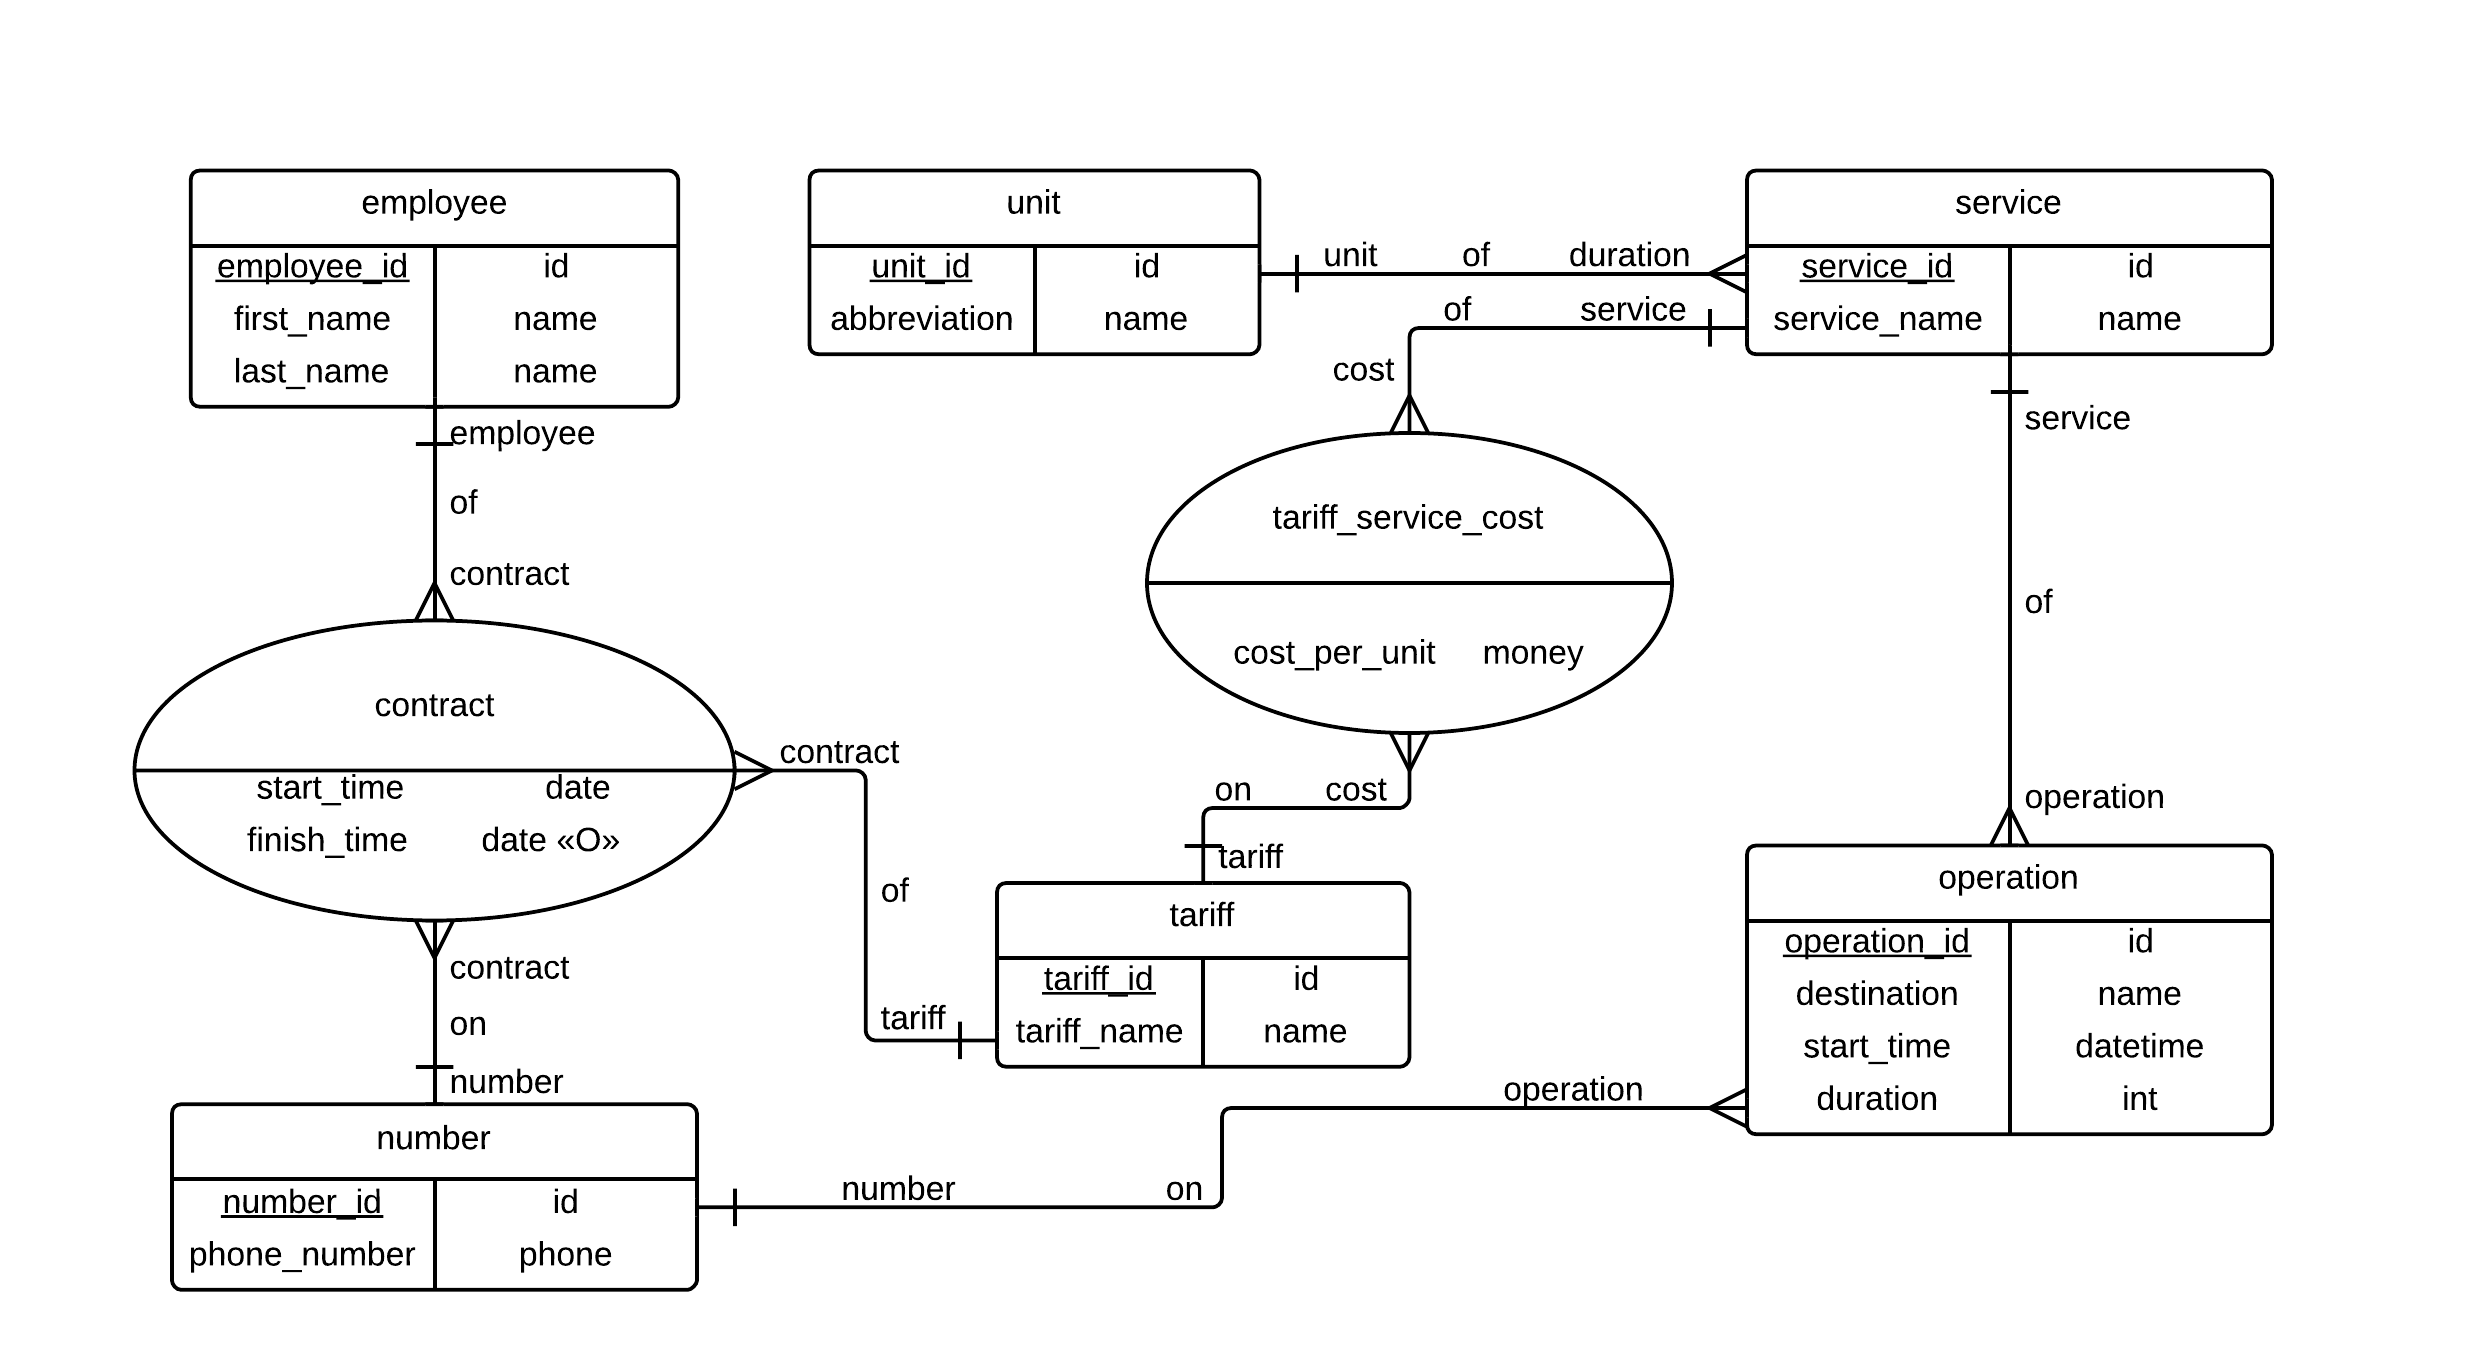
\includegraphics[scale=0.2]{erm}
	\caption{Модель сущность-связь}
	\label{fig:erm}
\end{figure}

\begin{figure}[H]
	\centering
	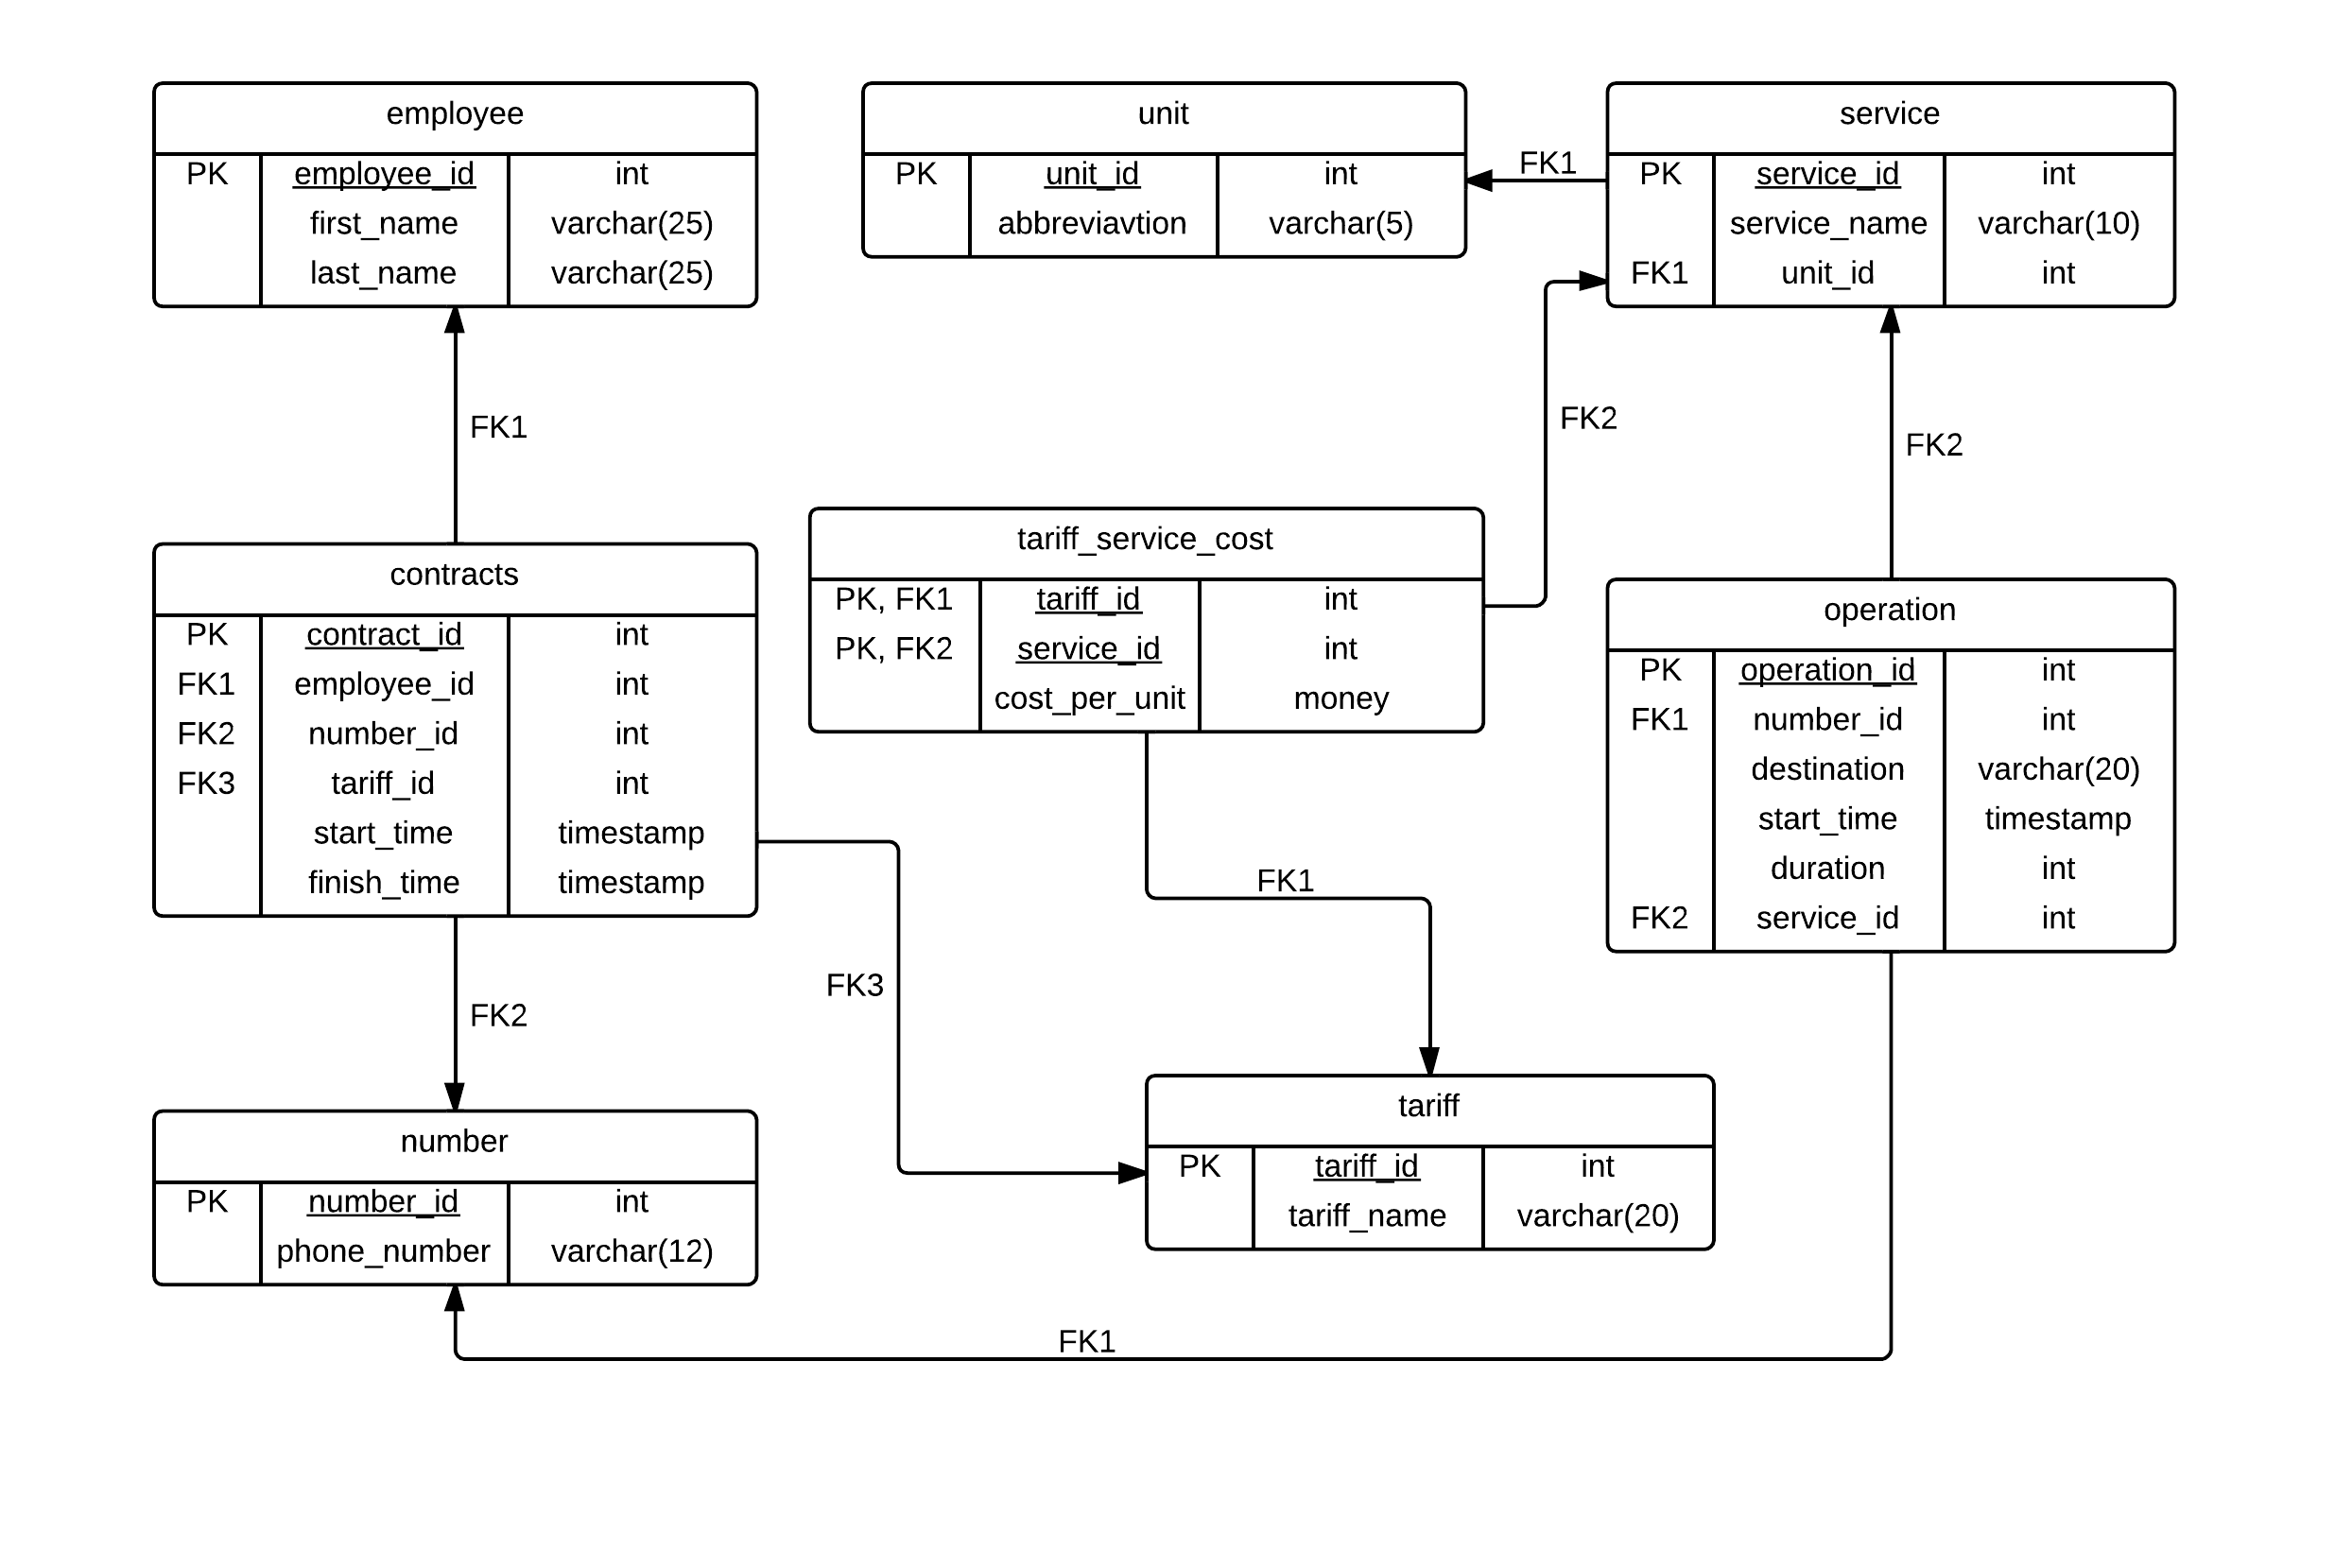
\includegraphics[scale=0.2]{pdm}
	\caption{Физическая модель}
	\label{fig:pdm}
\end{figure}

\end{document}
